\chapter{Problem Definition}

The emerging need of image processing techniques in everyday life is inevitable. There have been lots of image processing algorithms proposed to increase the overall availability of tools in image understanding and using these tools to improve the human life. \textit{Template Matching} is a task that its applications are obvious in everyday life. Computer vision tasks such as \textit{object detection}, \textit{object recognition} and other tasks based on these two main questions; Is there a certain object in the image? And if yes, where is it in the image?, can be classified as subproblems of \textit{template matching} task. This task can be extended to counting the number of occurrences of an object in a given image. Given a main image and a template image, we want to find occurrences of the template image in main image. This problem can be solved in many ways. In the next chapter, we'll analyze the procedure of \textit{naive} template matching to solve this problem. In further chapters, we'll provide the procedure of using \textit{Fast Fourier Transform} to convert the images into frequency domain. We'll show that finding the maximum value of the result of the convolution of two images is where the template has occurred in main image.

\section{Naive Template Matching}
The main task of naive template matching was clearly explained in the previous section. There are various similarity measures in naive template matching. The one we use here is \textit{SAD} or \textit{Sum of Absolute Deviations} which is formally described further. Let $f$ and $t$ be the main image and the template image respectively and $(x, y)$ represent the column and the row of each image. The \textit{Sum of Absolute Deviations} error metric for two images can be written as:
\begin{equation}
	SAD = \sum_{x, y}^{}f(x, y) - t(x - u, y - v)
\end{equation}

Note that there is also a more precise error metric called \textit{Sum of Squared Errors} which is represented as:
\begin{equation}
		SSD = \sum_{x, y}^{}[f(x, y) - t(x - u, y - v)]^2
\end{equation}
In this project, we'll use the first error metric because of the processing power limits.

\section{FFT-Based Template Matching}
\subsection{One-Dimensional Discrete Fourier Transform}
The Fourier transform of a discrete function of one variable, $f(x)$, $x = 0, 1, 2, ..., M-1$, is given by the equation
\begin{equation}
	F(u) = \frac{1}{M}\sum_{x = 0}^{M - 1} f(x) e^{-j2\pi ux/M} \ \ \ \ u = 0, 1, 2, ..., M-1
\end{equation}
Similarly, given $F(u)$, we can obtain the original function back using the inverse DFT:
\begin{equation}
	f(x) = \sum_{u = 0}^{M -1}F(u)e^{j2\pi ux /M} \ \ \ \ x = 0, 1, 2, ..., M - 1
\end{equation}
\subsection{Two-Dimensional Discrete Fourier Transform}
Extension of the one-dimensional discrete Fourier transform and its inverse to two dimensions is straightforward. The discrete Fourier transform of a function (image) $f(x, y)$ of size $M * N$ is given by the equation
\begin{equation}
	F(u, v) = \frac{1}{MN}\sum_{x = 0}^{M - 1}\sum_{y = 0}^{N - 1}f(x, y)e^{-j2\pi(ux/M + ry/N)}
\end{equation}
As in the 1-D case, this expression must be computed for values of $u = 0, 1, 2, ..., M -1 $, and also for $v = 1, 2, ..., N -1 $. Similarly, given $F(u, v)$, we obtain $f(x, y)$ via the inverse Fourier transform, given by the expression
\begin{equation}
	f(x, y) = \sum_{u = 0}^{M -1}\sum_{r = 0}^{N - 1} F(u, v)e^{j2\pi (ux/M + ry/N)}
\end{equation}

\subsection{Convolution and Correlation Theorems}
The discrete convolution of two functions $f(x, y)$ and $h(x, y)$ of size $ M * N$ is denoted by $f(x, y) \star h(x, y)$ and is defined by the expression
\begin{equation}
	f(x, y) \star h(x, y) = \frac{1}{MN}\sum_{m = 0}^{M - 1}\sum_{n = 0}^{N - 1}f(m, n)h(x - m, y-m)
\end{equation}
we also know that the convolution theorem consists of the following relationships between the two functions and their Fourier transforms:
\begin{equation}
	f(x, y) \star h(x, y) \leftrightarrow F(u, v)H(u, v)
\end{equation}
and 
\begin{equation}
	f(x, y)h(x, y) \leftrightarrow F(u, v) \star H(u, v)
\end{equation}
The correlation of two functions $f(x, y)$ and $h(x, y)$ is defined as
\begin{equation}
	f(x, y)\circ h(x, y) = \frac{1}{MN} \sum_{m = 0}^{M - 1}\sum_{n = 0}^{N - 1}f^*(m, n)h(x + m, y + n)
\end{equation}
where $f^*$ denotes the complex conjugate of $f$. Convolution is the tie between filtering in the spatial and frequency domains. The principal use of correlation is for matching. In matching, $f(x, y)$ is an image containing objects or regions. If we want to determine whether $f$ contains a particular object or region in which we are interested, we let $h(x, y)$ be that object or region (we call this image a template). Then, if there is a match, the correlation of two functions will be maximum  at the location where $h$ finds a correspondence in $f$. An example of this phenomenon is provided in figure 2.1.
\begin{figure}[!h]\centering
	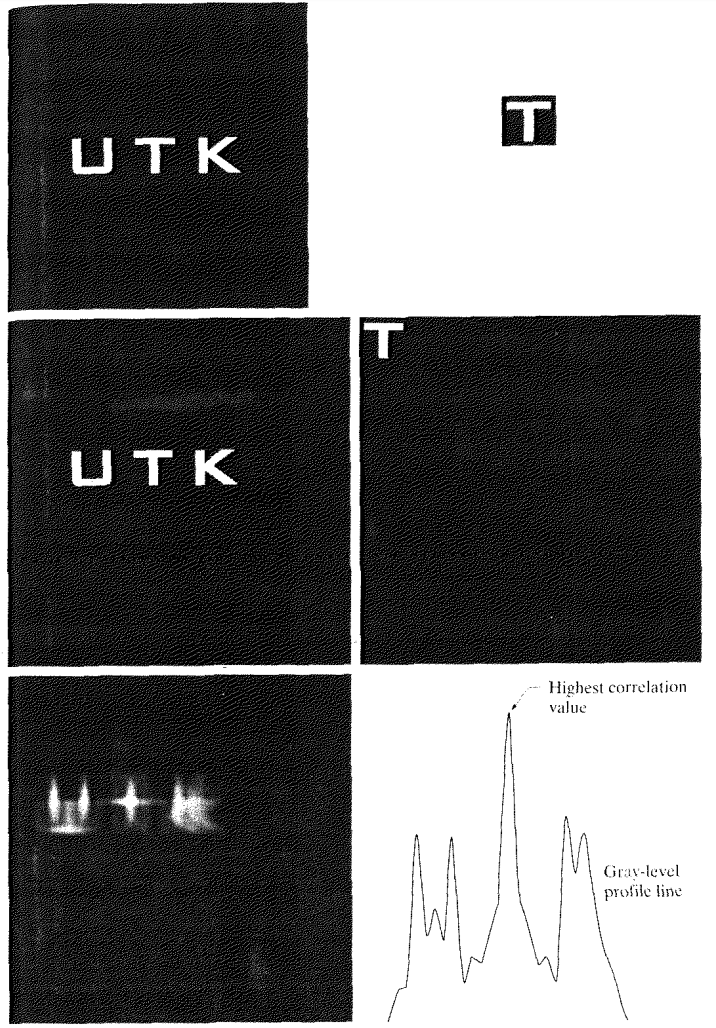
\includegraphics[width=0.8\textwidth]{figure_2_1.PNG}
	\caption{Illustration of image padding and correlation. The highest value of the correlation function occurs at the point where template is exactly on top of the \textit{T} in the image.}
	\label{pl1}
\end{figure}

\section{Fast Fourier Transform}
One of the main reasons that the DFT has became an essential tool in signal processing was the development of the fast Fourier transform. Computing the 1-D Fourier transform of $M$ points requires on the order of $M^2$ multiplication/addition operations. The FFT accomplishes the same task on the order of $M \log_2 M $ operations. If, for example $M = 1024$, the brute-force method will require approximately $10^6$ operations. While the FFT will require approximately $10^4$ operations. This is a computational advantage of 100 to 1. The decrease in computational complexity significantly impacts the time needed for processing the images. The FFT algorithm is based on the so-called \textit{successive doubling method}. Let's define the equation
\begin{equation}
	F(u) = \frac{1}{M} \sum_{x = 0}^{M - 1}f(x)W_M^{ux}
\end{equation}
where 
\begin{equation}
	W_M = e^{-j2\pi / M}
\end{equation}
and $M$ is assumed to be of the form
\begin{equation}
	M = 2^n
\end{equation}
with $n$ being a positive integer. Hence, $M$ can be expressed as 
\begin{equation}
	M = 2K
\end{equation}
Substitution of (2.14) into (2.11) yields
\begin{equation}
	F(u) = \frac{1}{2}[\frac{1}{K}\sum_{x = 0}^{K - 1} f(2x)W^{u(2x)}_{2K} + \frac{1}{K}\sum_{x = 0}^{K - 1}f(2x + 1)W_{2k}^{u(2x + 1)}]
\end{equation}
The number of multiplications and additions required to implement FFT:
\begin{equation}
	m(n) = 2m(n - 1) + 2^{n - 1} \ \ \  n \geq 1 = \frac{1}{2} M \log_2 M
\end{equation}
and
\begin{equation}
	a(n) = 2a(n - 1) + 2^n  \ \ \ n \geq 1 = M \log_2 M
\end{equation}